\documentclass[a4paper]{article}

\usepackage[english]{babel}
\usepackage[utf8]{inputenc}
\usepackage{amsmath}
\usepackage{amssymb}
\usepackage{caption}
\usepackage{siunitx}
\usepackage{graphicx}
\usepackage{textcomp}
\usepackage{gensymb}
\graphicspath{{./}}
\usepackage[colorinlistoftodos]{todonotes}
\usepackage[section]{placeins}
\setlength{\parindent}{0pt}
\usepackage{url}
\usepackage{bm}
\usepackage{mathtools}
\usepackage{enumerate}

\def\rcurs{{\mbox{$\resizebox{.09in}{.08in}{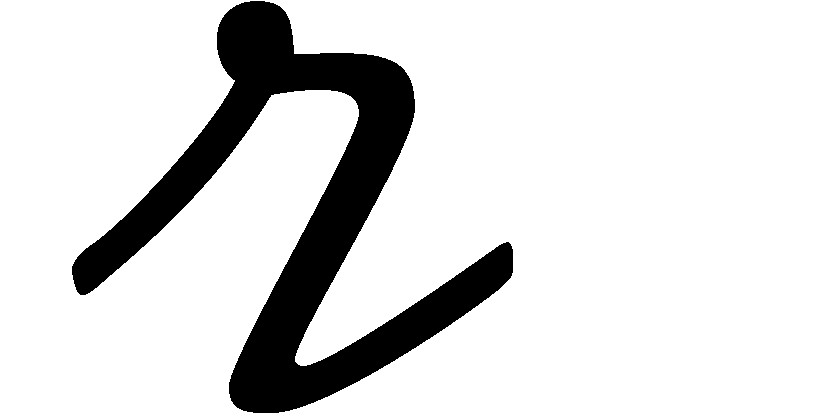
\includegraphics[trim= 1em 0 14em 0,clip]{ScriptR}}$}}}
\def\brcurs{{\mbox{$\resizebox{.09in}{.08in}{
\includegraphics[trim= 1em 0 14em 0,clip]{BoldR}}$}}}
% \def\rcurs{{\mbox{$\resizebox{.16in}{.08in}{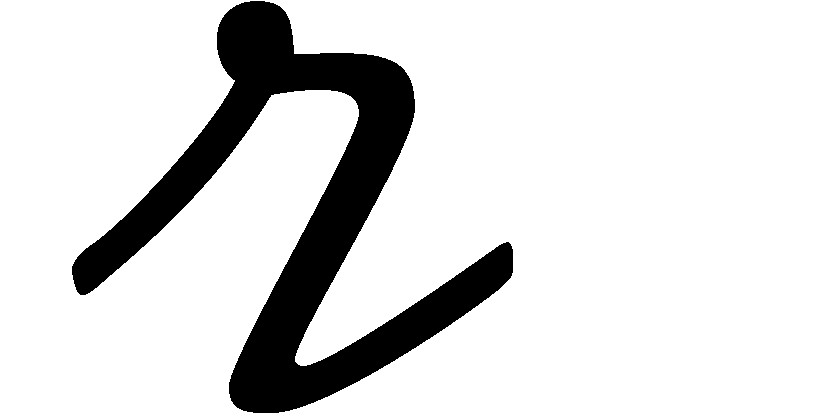
\includegraphics{ScriptR}}$}}}
% \def\brcurs{{\mbox{$\resizebox{.16in}{.08in}{
\includegraphics{BoldR}}$}}}
\def\hrcurs{{\mbox{$\hat \brcurs$}}}

\title{Lecture Notes E\&M}
\author{Mick Veldhuis}
\date{\today}

\begin{document}
\maketitle

\tableofcontents

\section{Chapter 1: Vector calculus}

\subsection{Gradient, divergence and the curl}
(1) The gradient is the vector derivative of a scalar (function) such as $T(x, y, z)$, then $\nabla T$ will be the gradient of $T$, which is a vector pointing in the direction of maximum increase.

\bigskip

(2) The divergence of a vector function is a measure of the spread of a vector field and is denoted by $\nabla \cdot \bm{v}$.

\bigskip

(3) The curl of a vector field is the swirl around the point in question and is denoted by $\nabla \times \bm{v}$.

\subsection{Fundamental theorems of vector calculus}
First, the fundamental theorem of gradients:
\begin{equation}
    \int_{a}^{b} \nabla T\cdot d\bm{l} = T(b) - T(a)
\end{equation}1

Which implies that $\oint \nabla T\cdot d\bm{l}=0$. Secondly, the Gauss's theorem (or Green's theorem, Gauss's theorem in 2D):
\begin{equation}
    \int_V (\nabla \cdot \bm{v}) \,d\tau = \oint_S \bm{v} \cdot d\bm{a}
\end{equation}
And thirdly, Stokes theorem:
\begin{equation}
    \int_S (\nabla \times \bm{v}) \cdot d\bm{a} = \oint_P \bm{v}\cdot d\bm{l}
\end{equation}
Which implies that the left hand only depends on the boundary and not the surface, and that $\oint_S (\nabla \times \bm{v}) \cdot d\bm{a}=0$ for any closed surface. Note that $d\bm{a}$ depends on the path, to obtain the direction use the right hand rule.

\subsection{The Dirac delta function}
The Dirac delta function is a distribution defined as follows in 1D:

\[f(x) = \left\{
  \begin{array}{lr}
    0 & \text{if}\ x \not= 0\\
    \infty & \text{if}\ x = 0
  \end{array}
\right.
\]

such that

\begin{equation}
    \int_{-\infty}^{\infty} f(x)\delta(x)dx=f(0)
\end{equation}

So for $\delta(x-a)$, under the integral, the delta function will pick out the function $f(x)$ at $x=a$. A handy rule to remember is:

\begin{equation}
    \delta(kx)=\frac{1}{|k|}\delta(x)
\end{equation}

In 3D the delta function would be defined with $\delta^3(\bm{r})=\delta(x)\delta(y)\delta(z)$ such that

\begin{equation}
    \int f(\bm{r})\delta^3(\bm{r}-\bm{a})d\tau = f(\bm{a})
\end{equation}

The following relation is handy to remember:

\begin{equation}
    \nabla\cdot \bigg(\frac{\hat{r}}{r^2}\bigg)=4\pi\delta^3(\bm{r})
\end{equation}

\section{Chapter 2: Electrostatics}

\subsection{Coulombs law}
The force on a test charge $Q$ due to a point charge $q$ is given by:
\begin{equation}
    \bm{F}=\frac{1}{4\pi\epsilon_0}\frac{qQ}{\rcurs^2}
\end{equation}

such that $\bm{F}=Q\bm{E}$, where $\brcurs=\bm{r}-\bm{r'}$.

Then we can generalize the electric field $\bm{E}$ of a distribution of charges as follows:

\begin{equation}
    \bm{E}=\frac{1}{4\pi\epsilon_0}\int \frac{\hat{\brcurs}}{\rcurs^2}dq
\end{equation}

where $dq$ is either $\lambda dl'$,  $\sigma da'$ or $\rho d\tau'$ depending on nature of the distribution of charges.

\subsection{Gauss's law}
We can more easily calculate the electric field by applying Gauss's law which states that
\begin{equation}
    \oint \bm{E}\cdot d\bm{a} = \frac{Q_{enc}}{\epsilon_0}
\end{equation}

Where $Q_{enc}=\int \,dq$.This law can be applied in the case of spherical, cylindrical or plane symmetry. We can also easily obtain the differential form of Gauss's law, namely $\nabla\cdot \bm{E}$:
\begin{equation}
    \nabla\cdot\bm{E}=\frac{\rho}{\epsilon_0}
\end{equation}

And it is important to note that in the case of electrostatics we have that $\nabla\times \bm{E}=0$.

\subsection{The electric potential}
The potential, defined w.r.t. to a reference points $O$ such that $V(\bm{r})$ is given as

\begin{equation}
    V(\bm{r})=-\int_{O}^{r} \bm{E}\cdot d\bm{l}
\end{equation}

Mostly $O$ will be set at $\infty$, but will be arbitrary if the charge distribution itself will extend to infinity. With the potential we can also easily calculate the electric field, namely by $\bm{E}=-\nabla V$. We can now also determine Poisson's equation, which is simply the laplacian of $V\Rightarrow \nabla^2V=-\rho/\epsilon_0$. The Electric potential for continuous charge distributions yields:

\begin{equation}
    V(\bm{r})=\frac{1}{4\pi\epsilon_0}\int \frac{dq}{\rcurs} 
\end{equation} 

\subsection{The work done on charges}
For a single charge we simply obtain:
\begin{equation}
    W=\int_{a}^{b}\bm{F}\cdot d\bm{l}=-Q\int_{a}^{b} \bm{E}\cdot d\bm{l}=Q[V(b)-V(a)]
\end{equation}

If you want to bring a charge $Q$ from $\infty$ we would obtain $W=QV(\bm{r})$. For a multiple of charges the energy to assemble the configuration would be:
\begin{equation}
    W = \frac{1}{2}\sum_{i=1}^{n}q_i\bigg(\sum_{j\not=i}^{n}\frac{1}{4\pi\epsilon_0}\frac{q_j}{\rcurs_{ij}}\bigg)=\frac{1}{2}\sum_{i=1}^{n}q_iV(\bm{r}_i)
\end{equation}

\subsection{The energy of a continuous charge distribution}
Generally it would be
\begin{equation}
    W=\frac{1}{2}\int V\,dq
\end{equation}

But this is not very practical, so we can rewrite it as

\begin{equation}
    W=\frac{\epsilon_0}{2}\bigg(\int_V E^2\, d\tau+\oint_S V\bm{E}\cdot d\bm{a}\bigg)
\end{equation}

And this can be simplified to

\begin{equation}
    W=\frac{\epsilon_0}{2}\int_{V} E^2\, d\tau
\end{equation}

where $V$ implies all space.

\subsection{Conductors}
Conductors are materials in which electrons can move freely, and the following statements apply to all conductors:

\begin{enumerate}
    \item $\bm{E}=0$ inside the conductor, since a field inside the conductor would be caused by an outside field which is opposite to the internal field and the inside field cancels with the outside field. 
    \item $\rho=0$ inside the conductor, this follows from the differential form of Gauss's law for $\bm{E}=0$.
    \item Any charge resides on the surface of the conductor.
    \item A conductor is equipotential, meaning for any points $a$ and $b$ we have $V(a)=V(b)$ since $\int \bm{E}\cdot d\bm{l}=0$.
    \item $\bm{E}$ is perpendicular to the surface just outside the conductor.
\end{enumerate}

\subsection{Capacitors}
A capacitor consists of two conductors with a vacuum (or dielectric) that separates the two, often we apply a charge $Q$ to one and $-Q$ to the other plate. The effect of such a capacitor is the capacitance defined as

\begin{equation}
    C \equiv \frac{Q}{V}
\end{equation}

Where $C$ is measured in farads ($F$) and it is intrinsically positive. 

\bigskip

We can charge a capacitor by removing electrons from the positive plate, the work done to charge the capacitor would then be

\begin{equation}
    W=\frac{1}{2}CV^2
\end{equation}

\section{Chapter 3: Approximating potentials and fields}
We can approximate the electric field and potential by applying multipole expansion. The first two terms of that expansion will be discussed here.
\subsection{The monopole term}
For the first term we have 

\begin{equation}
    V_{mon}(\bm{r})=\frac{1}{4\pi\epsilon_0}\frac{Q}{r}
\end{equation}

where $Q$ is the monopole moment, the sum of all charges (in the case of point charges). A pure monopole would be a point charge at the origin.

\subsection{The dipole term}
The second term, would be

\begin{equation}
    V_{dip}(\bm{r})=\frac{1}{4\pi\epsilon_0}\frac{\bm{p}\cdot\hat{\bm{r}}}{r^2},\ \bm{p} \equiv \int \bm{r}'\rho(\bm{r}')d\tau'
\end{equation}

Or in the case of point charges $\bm{p}=\sum q_i \bm{r}_i'$. A pure dipole would in turn be defined as a distribution for which $q\rightarrow \infty$ and for which the distance between charges goes to zero. We can now calculate $\bm{E}_{dip}$, this is done by rewriting equation \textbf{[22]} and using that $\bm{E}=-\nabla V$:

\begin{equation}
    V_{dip}(r, \theta)=\frac{\hat{\bm{r}}\cdot\bm{p}}{4\pi\epsilon_0 r^2}=\frac{p\cos\theta}{4\pi\epsilon_0 r^2}\ \Rightarrow\ \bm{E}_{dip}=\frac{p}{4\pi\epsilon_0 r^3}(2\cos\theta\hat{\bm{r}}+\sin\theta\hat{\bm{\theta}})
\end{equation}

\section{Chapter 4: Electric fields in matter}

\subsection{Atomic polarizability}

If a polar atom is placed in an electric field it will get a dipole moment: $\bm{p}=\alpha\bm{E}$. Where $\alpha$ is the proportionality constant.

\subsection{Polar molecules}

Polar molecules in an external electric field experience a torque $\bm{N}$. In a uniform field $\bm{N}=\bm{p}\times\bm{E}=q\bm{d}\times\bm{E}$. In a nonuniform field $\bm{N}=\bm{p}\times\bm{E}+\bm{r}\times\bm{F}$, with $\bm{F}=(\bm{p}\cdot\nabla)\bm{E}$.

\subsection{Polarization}

The polarization is the dipole moment per unit volume $\bm{P}=\frac{1}{V}\bm{p}$.

\subsection{Potential of a polarized object}

Given bound charges $\sigma_b=\bm{P}\cdot\bm{\hat{n}}$ and $\rho_b=-\nabla\cdot\bm{P}$ we obtain

\begin{equation}
    V=\frac{1}{4\pi\epsilon_0}\bigg[\oint \frac{\sigma_b}{\rcurs}da'+\int \frac{\rho_b}{\rcurs}d\tau'\bigg]
\end{equation}

\subsection{Gauss's law and dielectrics}

Within the dielectric the total chage density $\rho=\rho_f+\rho_b$, such that we obtain $\nabla\cdot (\epsilon_0\bm{E}+\bm{P})=\rho_f$, where $\bm{D}=\epsilon_0\bm{E}+\bm{P}$. So that $\nabla\cdot\bm{D}=\rho_f$, in the end we can define the following

\begin{equation}
    \oint \bm{D}\cdot d\bm{a}=Q_{fenc}
\end{equation}

\subsection{Linear dielectrics}

A linear dielectric obeys $\bm{P}=\epsilon_0\chi_e\bm{E}$, where $\chi_e$ is the electric susceptibility. We can define $\bm{D}$, but now as

\begin{equation}
    \bm{D}=\epsilon_0\bm{E}+\bm{P}=\epsilon_0 (1+\chi_e)\bm{E}=\epsilon\bm{E}
\end{equation}

where $\epsilon$ is the permittivity. We can define the dielectric constant $\epsilon_r=1+\chi_e=\epsilon/\epsilon_0$.

\bigskip

In space containing a homogeneous linear dielectric we have $\bm{D}=\epsilon_0\bm{E}_{vac}$, so that $\bm{E}=\bm{D}/\epsilon=\bm{E}_{vac}/\epsilon_r$.


\subsection{The energy in a dielectric system}

\begin{equation}
    W=\frac{1}{2}\int \bm{D}\cdot\bm{E}\,d\tau
\end{equation}

\subsection{Force in dielectrics}
\begin{equation}
    F=\frac{1}{2}V^2\frac{dC}{dx}
\end{equation}

\section{Chapter 5: Magnetostatics}

\subsection{Lorentz force law}
\begin{equation}
    \bm{F}_{m}=Q(\bm{v}\times\bm{B})\Rightarrow \bm{F}=\bm{F}_{e}+\bm{F}_m=Q[\bm{E}+\bm{v}\times\bm{B}]
\end{equation}

Note that $\bm{F}_m$ does not do work. And we can define the magnetic field around a wire as $\bm{B}=\bm{I}\times\bm{r}$.

\subsection{Currents}
We consider various types of currents due to various moving charge distributions, caused by the typical line, surface and volume charges.
\subsubsection*{Line currents}
We have $\bm{I}=\lambda\bm{v}$.
\subsubsection*{Surface currents}
Now we have a surface current $\bm{K}$,

\begin{equation}
    \bm{K}\equiv \frac{d\bm{I}}{dl_{\perp}}=\sigma\bm{v}
\end{equation}

where $dl_{\perp}$ is an infinitesimal length running parallel to the current.
\subsubsection*{Volume currents}
Lastly the volume current $\bm{J}$,
\begin{equation}
    \bm{J}\equiv \frac{d\bm{I}}{da_{\perp}}=\sigma\bm{v}\quad\Rightarrow\quad I=\int \bm{J}\cdot d\bm{a} 
\end{equation}
where $da_{\perp}$ is an infinitesimal area running parallel to the current.

\begin{equation}
    \nabla\cdot \bm{J}=-\frac{\partial\rho}{\partial t}=0\quad \text{(in the case of magnetostatics)}
\end{equation}

\subsection{Magnetic force}
The magnetic force is defined as

\begin{equation}
    \bm{F}_{m}=\int (\bm{v}\times\bm{B})\,dq
\end{equation}

for (i) line, (ii) surface , and (iii) volume currents $\bm{F}_{m}$ is given as


\begin{equation}
    (i)\quad I\int (d\bm{l}\times\bm{B})\quad (ii)\quad \int (\bm{K}\times\bm{B})\,da\quad (iii)\quad \int (\bm{J}\times\bm{B})\,d\tau
\end{equation}



\subsection{Biot-Savart law}
For line currents the law is as follows:

\begin{equation}
    \bm{B}(\bm{r})=\frac{\mu_0}{4\pi}\int \frac{\bm{I}\times \brcurs}{\rcurs^2}dl'=\frac{\mu_0I}{4\pi}\int \frac{d\bm{l}'\times \brcurs}{\rcurs^2}
\end{equation}

For surface and volume currents the law will be similar, namely:

\begin{equation}
    \bm{B}(\bm{r})=\frac{\mu_0}{4\pi}\int \frac{\bm{K}(\bm{r}')\times \brcurs}{\rcurs^2}da'\ \ \text{and}\ \   \bm{B}(\bm{r})=\frac{\mu_0}{4\pi}\int \frac{\bm{J}(\bm{r}')\times \brcurs}{\rcurs^2}d\tau'
\end{equation}

\subsection{Ampere's law}
Like Gauss's law we also have a convenient way to determine magnetic fields in the case of symmetry. For one can apply the following law for infinite wires, infinite solenoids, infinite planes and toroids. It is stated in as follows:

\begin{equation}
    \oint \bm{B}\cdot d\bm{l} = \mu_0 I_{enc}
\end{equation}

where $I_{enc}=\int \bm{J}\cdot d\bm{a}$ is the current enclosed by the chosen Amperian loop. The law's differential form is given as

\begin{equation}
    \nabla\times\bm{B}=\mu_0\bm{J}
\end{equation}

\subsection{Ampere's law cheat sheet}

\subsubsection*{Infinite wires}
\begin{equation}
    \oint \bm{B}\cdot d\bm{l} = \mu_0 I_{enc}\ \Rightarrow\ (2\pi s)B=\mu_0 I\ \Rightarrow\ \bm{B}=\frac{\mu_0 I}{2\pi s}\hat{\bm{\phi}}
\end{equation}
\subsubsection*{Infinite plane}
Consider a plane (at $z=0$)with surface current $\bm{K}=K\hat{\bm{x}}$ and an Amperian loop of length $L$, thus

\begin{equation}
    I_{enc}=\int K\,dl_{\perp} = KL
\end{equation}
\begin{equation}
    \oint \bm{B}\cdot d\bm{l} = \mu_0 I_{enc}\ \Rightarrow\ 2BL=\mu_0 K L \Rightarrow B = \frac{\mu_0 K}{2}
\end{equation}

Then by application of the right-hand rule we find $\bm{B}=-\mu_0 K/2\,\hat{\bm{y}}$ for $z>0$ and $\bm{B}=\mu_0 K/2\,\hat{\bm{y}}$ for $z<0$.

\subsubsection*{Infinite solenoid}
The solenoid consists of $n=N/L$ closely wound turns (each carrying a current $I$) per unit length. On a cylinder with radius $R$. We consider an Amperian loop of length $L$,

\begin{equation}
    \oint \bm{B}\cdot d\bm{l} = \mu_0 I_{enc}\ \Rightarrow\ BL=\mu_0KL=\mu_0nIL \ \Rightarrow\ B=\mu_0nI
\end{equation}

Such that we obtain $\bm{B}=\mu_0nI\,\hat{\bm{z}}$ for inside the solenoid and $\bm{B}=\bm{0}$ outside.
\subsubsection*{Toroids}
We consider a circular ring of ($N$) tightly wound wires carrying a current $I$, first we consider the inside of the toroid:

\begin{equation}
    \oint \bm{B}\cdot d\bm{l} = \mu_0 I_{enc}\ \Rightarrow\ (2\pi s)B=\mu_0 NI\ \Rightarrow\ \bm{B}=\frac{\mu_0 NI}{2\pi s}\hat{\bm{\phi}}
\end{equation}

And outside the toroid, similar to the solenoid, the magnetic field is zero.

\subsection{Magnetic vector potential}
Like the electric potential we define $\bm{A}$ such that $\bm{B}=\nabla\times\bm{A}$ (and $\nabla\cdot\bm{A}=0$), as such we obtain $\nabla^2\bm{A}=-\mu_0\bm{J}$. And we get vector potentials for line, surface, and volume to be

\begin{equation}
    \bm{A}=\frac{\mu_0}{4\pi}\int\frac{\bm{I}}{\rcurs}\,dl'\quad\bm{A}=\frac{\mu_0}{4\pi}\int\frac{\bm{K}(\bm{r}')}{\rcurs}\,da'\quad\bm{A}=\frac{\mu_0}{4\pi}\int\frac{\bm{J}}{\rcurs}\,d\tau'
\end{equation}

\subsection{Magnetic multipole expansion}
The magnetic monopole moment is always zero, as there are no magnetic monopoles. The magnetic dipole potential given a magnetic dipole moment $\bm{m}$ is 
 
\begin{equation}
    \bm{A}_{dip}=\frac{\mu_0}{4\pi r^2}\frac{\bm{m}\times\bm{\hat{r}}}{r^2}\quad\text{where}\quad\bm{m}\equiv I\int\,d\bm{a}=I\bm{a}
\end{equation}

so we obtain

\begin{equation}
    \bm{A}_{dip}=\frac{\mu_0}{4\pi r^2}\frac{m\sin\theta}{r^2}\bm{\hat{\phi}}\Rightarrow \bm{B}_{dip}=\frac{\mu_0m}{4\pi r^3}(2\cos\theta\,\bm{\hat{r}}+\sin\theta\,\bm{\hat{\theta}})
\end{equation}

\section{Chapter 6: Magnetic fields in matter}

\subsection{Types of magnets}

\begin{enumerate}
    \item Paramagnetism: $\bm{M}$ and $\bm{B}$ are parallel, it is due to electron spin.
    \item Diamagnetism: $\bm{M}$ and $\bm{B}$ are antiparallel, it is due to the orbital motion of electrons.
    \item Ferromagnetism: their $\bm{M}$ is retained even after the field is gone.
\end{enumerate}

\subsection{Torque on magnetic dipoles}

$\bm{N}=\bm{m}\times\bm{B}$, the torque $\bm{N}$ on a dipole $\bm{m}$ is caused by the field $\bm{B}$. This torque account for paramagnetism. As such the force on a dipole $\bm{m}$ in a field $\bm{B}$ is $\bm{F}=\nabla (\bm{m}\times\bm{B})$.

\subsection{Effect of $\bm{B}$ on atomic orbits}

The electrons will speed up/down depending on the orientation of the magnetic field. This is the cause of diamagnetism. It is a much weaker effect than paramagnetism.

\subsection{Magnetization}

\begin{equation}
    \bm{M}=\frac{1}{V}\bm{m}
\end{equation}

In general when someone places a diamagnet in a nonuniform magnetic field is repelled away and a paramagnet is atracted in to the field. 

\subsection{Bound currents}
We have

\begin{equation}
    \bm{J}_b=\nabla\times\bm{M}\quad\text{and}\quad\bm{K}_b=\bm{M}\times\bm{\hat{n}}
\end{equation}

such that

\begin{equation}
    \bm{A}=\frac{\mu_0}{4\pi}\bigg[\int\frac{\bm{J}_b}{\rcurs}\,d\tau'+\oint\frac{\bm{K}_b}{\rcurs}da'\bigg]
\end{equation}

\subsection{Ampere's law and magnetic materials}
We found that in magnetic materials Ampere's law is given as

\begin{equation}
    \nabla\times (\frac{1}{\mu_0}\bm{B}-\bm{M})=\bm{J}_f
\end{equation}

we define $\bm{H}$, the auxiliary field, such that we have $\nabla\times\bm{H}=\bm{J}_f$,

\begin{equation}
    \oint\bm{H}\cdot d\bm{l}=I_{fenc}
\end{equation}

\subsection{Linear media}
Linear media obey $\bm{M}=\chi_m\bm{H}$, where $\chi_m$ is the magnetic susceptibility. Such that 

\begin{equation}
    \bm{B}=\mu_0(\bm{H}+\bm{M})=\mu_0(1+\chi_m)\bm{H}=\mu\bm{H}
\end{equation}

In a vacuum $\bm{H}\rightarrow 0$. If $\chi_m > 0$ we are talking about paramagnetism and if $\chi_m < 0$ we are talking about diamagnetism. The volume bound current density in a homogeneous linear material is given as $\bm{J}_b=\nabla\times\bm{M}=\chi_m\bm{J}_f$.

\subsection{Ferromagnetism}

It is caused by the unpaired electron spin aligning in patterns called domains. 

To make a permanent magnet, apply a (strong) magnetic field such that a torque will be exerted. And domain boundaries will grow, if they are initially close to parallel with the magnetic field. Else they will shrink. If one domain totally overtakes we call it saturated.

\section{Chapter 7: Electrodynamics}

\subsection{Ohms law}
The current density ($\bm{J}$) is proportional to the force per unit charge ($\bm{f}$):
\begin{equation}
    \bm{J}=\sigma\bm{f}
\end{equation}

where $\sigma$ is the conductivity (theoretically for a perfect conductor $\sigma=\infty$; insulator $\sigma=0$). Often the resistivity ($\rho$) is used $\rho = 1 / \sigma$. Often the force is the em-force that does the job so $\bm{J}=\sigma(\bm{E}+\bm{v}\times\bm{B})$, when $v<<c$ we can just say $\bm{J}=\sigma\bm{E}$. 

\bigskip

The total current flowing from one electrode to the other is proportional to the potential difference between them; $V=IR$. Where $R$ is the resistance; it's a function of the geometry of the arrangement and the conductivity of the medium. 

\bigskip

If there are $n$ molecules per unit volume, and $f$ free electrons per molecule, each with charge $q$ and mass $m$, the current density is given as

\begin{equation}
    \bm{J}=nfq\bm{v}_{avg}=\frac{nfq\lambda}{2v_{thermal}}\frac{\bm{F}}{m}=\bigg(\frac{nf\lambda q^2}{2mv_{thermal}}\bigg)\bm{E}=\sigma\bm{E}
\end{equation}

where $\lambda$ is the distance between collisions. From this one can for instance see that the conductivity decreases with an increase in temperature. 

\bigskip

As a result of all the collisions with the lattice, the work done by the electrical force is converted into heat in the conductor/resistor. The power $P$ delivered is then 

\begin{equation}
    P=VI=I^2R
\end{equation}

Which is called the \textbf{Joule heating law}.

\subsection{The electromotive force}
The work done per unit charge to push the charges around is called the \textbf{electromotive force} (or \textbf{emf} for short) and is defined as

\begin{equation}
    \mathcal{E}\equiv \oint\bm{f}\cdot d\bm{l}\quad\text{where}\quad \bm{f}=\bm{f}_s+\bm{E}
\end{equation}

and for electrostatic fields ($\oint \bm{E}\cdot d\bm{l}=0$) we obtain $\mathcal{E}=\oint\bm{f}_s\cdot d\bm{l}$.

\subsection{Motional emf}
Basically the regular emf, but caused by moving a wire through a magnetic field (e.g. by using a generator), thus

\begin{equation}
    \mathcal{E}=\oint \bm{f}_{mag}\cdot d\bm{l}=vBh
\end{equation}

for a wire with width $h$. We can express this in a nicer way by defining the flux ($\Phi$) of $\bm{B}$ through the current loop:

\begin{equation}
    \Phi\equiv\int\bm{B}\cdot d\bm{a}
\end{equation}

such that we obtain the \textbf{flux rule} for motional emf,

\begin{equation}
    \mathcal{E}=-\frac{d\Phi}{dt}
\end{equation}

\subsection{Faraday's law}

Faraday did three experiments: (i) pulling a wire through a magnetic field, (ii) now holding the wire still and pulling the magnet to the opposite side, and (iii) changing the magnetic field, keeping the rest still.

\bigskip

Basically finding out that whenever and for whatever reason the $\Phi$ changes, an emf $\mathcal{E}$ will appear in the loop. From which the following equations were established:

\begin{equation}
    \nabla\times\bm{E}=-\frac{\partial\bm{B}}{\partial t}
\end{equation}

and in integral form we obtain,

\begin{equation}
    \oint\bm{E}\cdot d\bm{l}=-\int \frac{\partial\bm{B}}{\partial t}\cdot d\bm{a}=-\frac{d\Phi}{dt}=\mathcal{E}
\end{equation}

or alternatively if the surface does not change over time,

\begin{equation}
    \oint\bm{E}\cdot d\bm{l}=-\frac{d}{dt}\int\bm{B}\cdot d\bm{a}
\end{equation}

To keep track of the sign in Faraday's law we use a rule called \textbf{Lenz's law}: \textit{Nature abhors a change in flux}. Meaning that the induced current will flow in such a direction that it cancels the change in flux.

\bigskip

Note that in order to determine the direction of the induced $\bm{E}$, we deduce it from Faraday's law or by using that $\bm{E}\propto\brcurs\times\bm{B}$.

\subsection{Inductance}
If one has to wires at rest and one runs a steady current $I_1$ through loop one it will produce a magnetic field $B_1$ and a flux through loop two $\Phi_2$. We find that the magnetic field is proportional to the current and the flux therefore as well. Such that we obtain: $\Phi_2=M_{21}I_1$, where $M_{21}$ is called the mutual inductance of the two loops (note: $M_{21}=M_{12}$ so we will just use $M=M_{21}=M_{12}$). $M$ is a purely geometrical quantity that can be calculated by using the \textbf{Neumann formula}, that is not particularly practical:

\begin{equation}
    M=\frac{\mu_0}{4\pi}\oint\oint\frac{d\bm{l}_1\cdot d\bm{l}_2}{\rcurs}
\end{equation}

If one varies $I_1$ then an emf in the second loop $\mathcal{E}_2$ will be induced.

\begin{equation}
    \mathcal{E}_2=-\frac{d\Phi_2}{dt}=-M\frac{dI_1}{dt}
\end{equation}

It also produces an emf in its own wire, $\Phi=LI$, where $L$ is called the \textbf{self inductance} (or \textbf{inductance}) measured in henries. Inductance is intrinsically positive. So

\begin{equation}
    \mathcal{E}=-L\frac{dI}{dt}
\end{equation}

The greater $L$ is, the harder it is to change the current.

\subsection{Energy in magnetic fields}

The work done against the back emf to get a current going is given by

\begin{equation}
    W=\frac{1}{2}LI^2
\end{equation}

which we can turn into

\begin{equation}
    W=\frac{1}{2}\int (\bm{A}\cdot\bm{J})\,d\tau
\end{equation}

and eventually get to

\begin{equation}
    W_{mag}=\frac{1}{2\mu_0}\int_{all\ space}B^2\,d\tau
\end{equation}

\subsection{Maxwell's fix for Ampere's law}

Maxwell introduced an extra term to Ampere's law to fix the issues that arose. The fixed equation is given as

\begin{equation}
    \nabla\times\bm{B}=\mu_0\bm{J}+\mu_0\epsilon_0\frac{\partial\bm{E}}{\partial t}
\end{equation}

From this equation we can deduce that a changing electric field induces a magnetic field, like a changing magnetic field induces an electric field. The extra term is called the \textbf{displacement current} $\bm{J}_d\equiv \epsilon_0(\partial\bm{E}/\partial t)$. In integral form we have

\begin{equation}
    \oint \bm{B}\cdot d\bm{l}=\mu_0I_{enc}+\mu_0\epsilon_0\int \bigg(\frac{\partial\bm{E}}{\partial t}\bigg)\cdot d\bm{a}
\end{equation}

\subsection{Maxwell's equations}

Maxwell's equations in differential and integral form:

\begin{align}
    \nabla\cdot\bm{E}=\frac{1}{\epsilon_0}\rho\quad &\Leftrightarrow\quad\oint \bm{E}\cdot d\bm{a}=\frac{Q_{enc}}{\epsilon_0} \\
    \nabla\cdot\bm{B}=0\quad &\Leftrightarrow\quad\oint\bm{B}\cdot d\bm{a}=0 \\ 
    \nabla\times\bm{E}+\frac{\partial\bm{B}}{\partial t}=\bm{0}\quad &\Leftrightarrow\quad\oint \bm{E}\cdot d\bm{l}=-\frac{\partial}{\partial t}\int \bm{B}\cdot d\bm{a} \\
    \nabla\times\bm{B}-\mu_0\epsilon_0\frac{\partial\bm{E}}{\partial t}=\mu_0\bm{J}\quad &\Leftrightarrow\quad\oint \bm{B}\cdot d\bm{l}=\mu_0I_{enc}+\mu_0\epsilon_0\frac{\partial}{\partial t}\int \bm{E}\cdot d\bm{a}
\end{align}

\subsection{Maxwell's equations in matter}

Maxwell's equations in matter in differential and integral form are as follows: 

\begin{align}
    \nabla\cdot\bm{D}=\rho_{f}\quad &\Leftrightarrow\quad\oint \bm{D}\cdot d\bm{a}=Q_{f_{enc}} \\
    \nabla\cdot\bm{B}=0\quad &\Leftrightarrow\quad\oint\bm{B}\cdot d\bm{a}=0 \\ 
    \nabla\times\bm{E}=-\frac{\partial\bm{B}}{\partial t}\quad &\Leftrightarrow\quad\oint \bm{E}\cdot d\bm{l}=-\frac{\partial}{\partial t}\int \bm{B}\cdot d\bm{a} \\
    \nabla\times\bm{H}=\bm{J}_{f}+\frac{\partial\bm{D}}{\partial t}\quad &\Leftrightarrow\quad\oint \bm{H}\cdot d\bm{l}=I_{f_{enc}}+\frac{\partial}{\partial t}\int \bm{D}\cdot d\bm{a}
\end{align}

\subsection{Boundary conditions }

The fields $\bm{E}$, $\bm{B}$, $\bm{D}$, and $\bm{H}$ will generally be discontinuous at a boundary between different media, or at a surface that carries a charge density $\sigma$. As such we find that the component of $\bm{D}$ that is perpendicular to the interface is discontinuous as

\begin{equation}
    D_1^{\perp}-D_2^{\perp}=\sigma_f
\end{equation}

As are the parallel components of $\bm{H}$

\begin{equation}
    \bm{H}_1^{||}+\bm{H}_2^{||}=\bm{K}_f\times\bm{\hat{n}}
\end{equation}

On the other hand both the perpendicular components of $\bm{B}$ and the parallel components of $\bm{E}$ are continuous at the boundaries, such that we obtain

\begin{equation}
    B_1^{\perp}-B_2^{\perp}=0\quad\text{and}\quad \bm{E}_1^{||}+\bm{E}_2^{||}=0
\end{equation}

\section{Chapter 8: Conservation Laws}

\subsection{The continuity equation}

If the charge in a region has changed, then exactly that amount should have passed in or out through through the surface separating the region(s). As such we obtain the following equation for the local conservation of charge: 

\begin{equation}
    \frac{\partial \rho}{\partial t}=-\nabla\cdot\bm{J}
\end{equation}

\subsection{Poynting's theorem}

In the previous chapters we found expressions for the work done to get a current going against the back emf, and the work needed to assemble a static charge distribution. By combining those two equations we find that the total energy per unit volume is given as

\begin{equation}
    u=\frac{1}{2}\bigg(\epsilon_0E^2+\frac{1}{\mu_0}B^2\bigg)
\end{equation}

Now we would like to have an expression for the work done by the em-forces acting on the available charges (that will have moved). We then find a sort of \textit{work-energy theorem} of electrodynamics:

\begin{equation}
    \frac{dW}{dt}=-\frac{d}{dt}\int_V u\,d\tau - \oint_S \bm{S}\cdot d\bm{a}
\end{equation}

This is called \textbf{Poynting's theorem}. The first integral is the total energy of the fields, the second the energy that is transported out. This theorem says that the work done on the charges by the em-force is equal to the decrease in energy remaining in the fields, minus the the energy that flowed out through the surface. 

\bigskip

And $\bm{S}$ is called the \textbf{Poynting vector}. The energy per unit time, per unit area, transported by the fields, and it is defined as

\begin{equation}
    \bm{S}\equiv \frac{1}{\mu_0}\big(\bm{E}\times\bm{B}\big)
\end{equation}

Finally we find an expression for the continuity equation for energy, which expresses local conservation of electromagnetic energy:

\begin{equation}
    \frac{\partial u}{\partial t}=-\nabla\cdot\bm{S}
\end{equation}

\subsection{Forces on a moving distribution of charges}

The expression for all forces (per unit volume) on a moving distribution of charges is given as

\begin{align}
    \bm{f}&=\epsilon_0\bigg[(\nabla\cdot\bm{E})\bm{E}+(\bm{E}\cdot\nabla)\bm{E}-\frac{1}{2}\nabla(E^2)\bigg] \\
          &+ \frac{1}{\mu_0}\bigg[(\nabla\cdot\bm{B})\bm{B}+(\bm{B}\cdot\nabla)\bm{B}-\frac{1}{2}\nabla(B^2)\bigg] \\
          &- \epsilon_0\frac{\partial}{\partial t}(\bm{E}\times\bm{B})
\end{align}

Such that the total force is given by $\bm{F}=\int \bm{f}\,d\tau$. This expression is to be simplified by introducing the Maxwell stress tensor:

\begin{gather}
    \overleftrightarrow{\bm{T}}
    = 
    \begin{pmatrix}
        T_{xx}& T_{xy} & T_{xz}\\
        T_{yx} & T_{yy} & T_{yz}\\
        T_{zx} & T_{zy} & T_{zz}\\
    \end{pmatrix}
\end{gather}

Here the indices label the direction of the force on a surface, and the direction of the normal to that surface. The terms are given by

\begin{equation}
    T_{ij}\equiv \epsilon_0\bigg(E_iE_j-\frac{1}{2}\delta_{ij}E^2\bigg)+\frac{1}{\mu_0}\bigg(B_iB_j-\frac{1}{2}\delta_{ij}B^2\bigg)
\end{equation}

where 

\begin{equation}
    \delta_{ij}
    =
    \begin{dcases}
        1\ ,\ \ i=j \\
        0\ ,\ \ i\not=j \\
    \end{dcases}
\end{equation}

Thus $\delta_{ij}=0$ for the non-diagonal items.
Such that the total force over that surface is given as

\begin{equation}
    \bm{F}=\oint \overleftrightarrow{\bm{T}}\cdot d\bm{a}-\epsilon_0\mu_0\frac{d}{dt}\int\bm{S}\,d\tau
\end{equation}

Using this stress tensor we can also rewrite the expression for the force per unit volume:

\begin{equation}
        \bm{f} =\nabla\cdot\overleftrightarrow{\bm{T}} -\epsilon_0\mu_0\frac{\partial\bm{S}}{\partial t}
\end{equation}

\subsection{Conservation of momentum}

From the expression of the force we can obtain the following expression for the change of momentum per unit time,

\begin{equation}
    \frac{d\bm{p}_{mech}}{dt}=\oint \overleftrightarrow{\bm{T}}\cdot d\bm{a}-\epsilon_0\mu_0\frac{d}{dt}\int\bm{S}\,d\tau
\end{equation}

The momentum stored in the fields is (by the right integral) given as

\begin{equation}
    \bm{p}=\epsilon_0\mu_0\int\bm{S}\,d\tau
\end{equation}

and the left integral is the momentum per unit time flowing in through the surface. The momentum density in the fields is

\begin{equation}
    \bm{g}=\epsilon_0\mu_0\bm{S}=\epsilon_0(\bm{E}\times\bm{B})
\end{equation}

and the momentum flux transported by the fields is $-\overleftrightarrow{\bm{T}}$. And if the momentum in the volume considered is not changing, then

\begin{equation}
    \int\frac{\partial \bm{g}}{\partial t}\,d\tau=\int\nabla\cdot\overleftrightarrow{\bm{T}}\,d\tau\quad\Rightarrow\quad \frac{\partial \bm{g}}{\partial t}=\nabla\cdot\overleftrightarrow{\bm{T}}
\end{equation}

Which is the continuity equation for em-momentum, although the momenta are not conserved by themselves. 

\section{Chapter 9: Electromagnetic waves}

\subsection{The wave equation}

EM-waves are defined as a function $f(z, t)$, where $f$ is the displacement at a point $z$, at time $t$. In general waves have a form $f(z, t)=g(z-vt)$, for which

\begin{equation}
    \frac{\partial^2 f}{\partial z^2}=\frac{1}{v^2}\frac{\partial^2 f}{\partial t^2} \ \ , \ \ v=\sqrt{\frac{T}{\mu}}
\end{equation}

where $T$ is the tension and $\mu$ is the mass per unit length. But since the wave equation involves the square of $v$, $f(z, t)=h(z+vt)$ is also a valid solution. The difference is that for the first solution the wave moves in the positive $z$ direction and the latter one in the negative $z$ direction. As such the most general solution would actually be

\begin{equation}
    f(z, t)= g(z-vt) + h(z+vt)
\end{equation}

\subsection{Sinusoidal Waves}

\subsubsection*{Conventional notation}

Waves, such as

\begin{equation}
    f(z, t) = A\cos\big[k\big(z-vt\big)+\delta\big]
\end{equation}

are rather familiar. Here $A$ is the amplitude, the argument of the cosine is called the phase ($\delta$ is the phase constant, $0\le\delta\le 2\pi$). We can set the phase to zero and by solving for $z$ we obtain the central maximum. The number $k$ is the wave number, which is related to the wavelength as $\lambda=2\pi/k$. We define the period $T=2\pi/kv$, the frequency $\nu=1/T=v/\lambda$, and the angular frequency $\omega=2\pi \nu=kv$. Such that the wave expression can be rewritten as

\begin{equation}
    f(z, t) = A\cos\big[kz-\omega t + \delta]
\end{equation}

This wave travels to the right. If we want it traveling to the left we flip the sign of $k$. 

\subsubsection*{Complex notation}

We can rewrite the expression in a complex form with Euler's formula, such that we obtain

\begin{equation}
    f(z, t) = \Re\big[Ae^{i(kz-\omega t+\delta)}\big]
\end{equation}

Thus the complex wave function can be written as

\begin{equation}
    \Tilde{f}(z, t)\equiv \Tilde{A}e^{i(kz-\omega t)}\ \ , \ \ \Tilde{A}\equiv Ae^{i\delta}
\end{equation}

such that

\begin{equation}
    f(z, t) = \Re\big[\Tilde{f}(z, t)\big]
\end{equation}

\subsubsection*{Linear combinations of sinusoidal waves, using Fourier Transformations}

Using Fourier transformations we can rewrite the complex expression as

\begin{equation}
    \Tilde{f}(z, t) =\int_{-\infty}^{\infty} \Tilde{A}(k)e^{i(kz-\omega(k)t)}\,dk
\end{equation}

\subsection{Two types of waves}

\begin{enumerate}
    \item Transverse waves are waves for which the displacement is perpendicular to the direction of propagation. Such as (idealized) ocean waves.
    \item Longitudinal waves are waves for which the displacement from equilibrium is along the direction of propagation. They are compression waves.
\end{enumerate}

\subsection{Wave equations for $\bm{E}$ and $\bm{B}$}

Using maxwell's equations we can derive expressions for the wave equations for the electric and magnetic field. To obtain the results we apply the curl to respectively Faraday's and Ampere-Maxwell's law. Such that for the electric field obtain

\begin{equation}
    \nabla^2\bm{E}=\mu_0\epsilon_0\frac{\partial^2\bm{E}}{\partial t^2}
\end{equation}

And for the magnetic field:

\begin{equation}
    \nabla^2\bm{B}=\mu_0\epsilon_0\frac{\partial^2\bm{B}}{\partial t^2}
\end{equation}

These equations imply that empty space supports the propagation of EM-waves. And per the wave equation all EM-waves travel at the same speed, namely

\begin{equation}
    v=\frac{1}{\sqrt{\mu_0\epsilon_0}}=c\approx 3\cdot 10^8\ \si{\meter\per\second}
\end{equation}

\subsection{Monochromatic plane waves}

\textbf{Monochromatic plane waves} are sinusoidal EM-waves with a single frequency $\omega$ and have no $x$ and $y$ components, solely a $z$ component. Such that we have fields of the form

\begin{equation*}
    \Tilde{\bm{E}}(z, t) = \Tilde{\bm{E}_0}e^{i(kz-\omega t)}\quad\text{and}\quad\Tilde{\bm{B}}(z, t) = \Tilde{\bm{B}_0}e^{i(kz-\omega t)}
\end{equation*}

where $\Tilde{\bm{E}_0}$ and $\Tilde{\bm{B}_0}$ are the (complex) amplitudes, and $\omega=ck$. So EM-waves are transverse, such that

\begin{equation*}
    \Tilde{\bm{B}_0}=\frac{k}{\omega}(\hat{\bm{z}}\times\Tilde{\bm{E}_0})
\end{equation*}

So $\bm{E}$ and $\bm{B}$ are in phase and mutually perpendicular and $B_0=\frac{1}{c}E_0$. As the $z$ direction is not special, so we can generalize the wave equations. So we introduce the vector $\bm{k}$, the propagation vector (pointing in the direction of propagation), with the wave number $k$ as magnitude. So

\begin{align*}
    \Tilde{\bm{E}}(\bm{r}, t) &= \Tilde{E_0}e^{i(\bm{k}\cdot\bm{r}-\omega t)}\hat{\bm{n}}\\[1em]
    \Tilde{\bm{B}}(\bm{r}, t) &= \frac{1}{c}\Tilde{E_0}e^{i(\bm{k}\cdot\bm{r}-\omega t)}(\hat{\bm{k}}\times\hat{\bm{n}})=\frac{1}{c}\hat{\bm{k}}\times\Tilde{\bm{E}}
\end{align*}

Here $\hat{\bm{n}}$ is the polarization vector, it defines the plane of vibration, which is perpendicular to the direction of propagation.

\subsection{Energy and momentum in EM-waves}

We can rewrite the expression for $u$, given that $B^2=\frac{1}{c^2}E^2=\mu_0\epsilon_0E^2$:

\begin{equation*}
    u=\epsilon_0E^2=\epsilon_0E_0^2\cos^2(kz-\omega t+\delta)
\end{equation*}

Similarly we can rewrite $\bm{S}$ (the energy per unit area, per unit time), yielding

\begin{equation*}
    \bm{S}=c\epsilon_0E_0^2\cos^2(kz-\omega t+\delta)\hat{\bm{z}}=cu\hat{\bm{z}}
\end{equation*}

EM-waves also carry momentum, so that

\begin{equation*}
    \bm{g}=\frac{1}{c^2}\bm{S}=\frac{1}{c}u\hat{\bm{z}}
\end{equation*}

But as the waves vary with time, these quantities do not remain the same. Such that the average of these quantities are given as:

\begin{align*}
    \langle u\rangle &= \frac{1}{2}\epsilon_0E_0^2\\[1em]
    \langle \bm{S}\rangle &= \frac{1}{2}c\epsilon_0E_0^2\hat{\bm{z}}\\[1em]
    \langle \bm{g}\rangle &= \frac{1}{2c}\epsilon_0E_0^2\hat{\bm{z}}\\
\end{align*}

We can also define the average power per unit area transported by an EM-wave, the intensity: $I\equiv\langle\bm{S}\rangle$. As light falls on a perfect absorber, it delivers its momentum to the surface. Which is the radiation pressure, defined as

\begin{equation*}
    P=\frac{1}{A}\frac{\Delta p}{\Delta t}=\frac{\langle\bm{g}\rangle Ac\Delta t}{A\Delta t}=\frac{1}{2}\epsilon_0E_0^2=\frac{I}{c}
\end{equation*}

\subsection{EM-waves in matter}

We can rewrite Maxwell's equations in matter in the case for which no free charge is available and also for the case that $\epsilon$ and $\mu$ do not vary from point to point. From which we can deduce that EM-waves propagate through a linear homogeneous medium at a speed of

\begin{equation*}
    v=\frac{1}{\sqrt{\epsilon\mu}}=\frac{c}{n}\quad\text{where}\quad n\equiv\sqrt{\frac{\epsilon\mu}{\epsilon_0\mu_0}}
\end{equation*}

where $n$ is called the index of refraction of the substance the wave is traveling through. If $\mu\approx\mu_0$, then $n\approx\sqrt{\epsilon_r}$. Then we can rewrite the expressions for $u$, $\bm{S}$, and $I$, to be valid in matter. Such that we obtain, noting that in matter $\omega=kv$,

\begin{align*}
    u&=\frac{1}{2}\bigg(\epsilon E^2+\frac{1}{\mu}B^2\bigg)\\[1em]
    \bm{S}&=\frac{1}{\mu}(\bm{E}\times\bm{B})\\[1em]
    I&=\frac{1}{2}\epsilon vE_0^2
\end{align*}

\subsection{Reflection and refraction of waves}

By the boundary conditions established in chapter 7, we obtain the phenomena of reflection and refraction of EM-waves. Suppose that if the $xy$-plane forms a boundary between to linear media. And a plane wave with frequency $\omega$, which travels in the $z$ direction and is polarized in the $x$ direction, that approaches the interface from the left will have wave equations

\begin{align*}
    \Tilde{\bm{E}}_I(z, t) = \Tilde{E}_{0_{I}}e^{i(k_1z-\omega t)}\hat{\bm{x}}\quad\text{and}\quad
    \Tilde{\bm{B}}_I(z, t) = \frac{1}{v_1}\Tilde{E}_{0_{I}}e^{i(k_1z-\omega t)}\hat{\bm{y}}
\end{align*}

Which gives rise to a reflected wave, that travels in the opposite direction as the original wave, 

\begin{align*}
    \Tilde{\bm{E}}_R(z, t) = \Tilde{E}_{0_{R}}e^{i(-k_1z-\omega t)}\hat{\bm{x}}\quad\text{and}\quad
    \Tilde{\bm{B}}_R(z, t) = -\frac{1}{v_1}\Tilde{E}_{0_{R}}e^{i(-k_1z-\omega t)}\hat{\bm{y}}
\end{align*}

And a transmitted wave, which continues to the right:

\begin{align*}
    \Tilde{\bm{E}}_T(z, t) = \Tilde{E}_{0_{T}}e^{i(k_2z-\omega t)}\hat{\bm{x}}\quad\text{and}\quad
    \Tilde{\bm{B}}_T(z, t) = -\frac{1}{v_2}\Tilde{E}_{0_{T}}e^{i(k_2z-\omega t)}\hat{\bm{y}}
\end{align*}

So there are no components perpendicular to the $xy$-plane, such that the boundary conditions require that

\begin{equation*}
    \Tilde{E}_{0_{I}}+\Tilde{E}_{0_{R}}=\Tilde{E}_{0_{T}}
\end{equation*}

and that

\begin{equation*}
    \Tilde{E}_{0_{I}}-\Tilde{E}_{0_{R}}=\beta\Tilde{E}_{0_{T}}\quad\text{where}\quad \beta\equiv\frac{\mu_1v_1}{\mu_2v_2}=\frac{\mu_1n_2}{\mu_2n_1}
\end{equation*}

Then solving for $\Tilde{E}_{0_{R}}$ and $\Tilde{E}_{0_{T}}$ yields:

\begin{equation*}
    \Tilde{E}_{0_{R}}=\bigg(\frac{1-\beta}{1+\beta}\bigg)\Tilde{E}_{0_{I}}\quad\text{and}\quad\Tilde{E}_{0_{T}}=\bigg(\frac{2}{1+\beta}\bigg)\Tilde{E}_{0_{I}}
\end{equation*}

We would like to know what fraction of the incident energy is reflected, and what fraction is transmitted. We have that $I=\frac{1}{2}\epsilon vE_0^2$, and if $\mu_1=\mu_2=\mu_0$, then the ratio of the reflected intensity to the incident intensity is

\begin{equation*}
    R\equiv\frac{I_R}{I_I}=\bigg(\frac{n_1-n_2}{n_1+n_2}\bigg)^2
\end{equation*}

and the ratio of the transmitted intensity to the incident intensity is

\begin{equation*}
    T\equiv\frac{I_T}{I_I}=\frac{4n_1n_2}{(n_1+n_2)^2}
\end{equation*}

Here $R$ is the \textbf{reflection coefficient} and $T$ is the \textbf{transmission coefficient}. And note that

\begin{equation*}
    R+T=1
\end{equation*}

\subsection{Reflection and transmission at oblique incidence}

Let's assume waves of the form

\begin{align*}
    \Tilde{\bm{E}}_I(\bm{r}, t) = \Tilde{\bm{E}}_{0_{I}}e^{i(\bm{k}_I\cdot\bm{r}-\omega t)}\quad\text{and}\quad\Tilde{\bm{B}}_I(\bm{r}, t) = \frac{1}{v_1}(\hat{\bm{k}}_I\times\Tilde{\bm{E}}_I)
\end{align*}

Such that the reflected and transmitted waves are

\begin{align*}
    \Tilde{\bm{E}}_R(\bm{r}, t) = \Tilde{\bm{E}}_{0_{R}}e^{i(\bm{k}_R\cdot\bm{r}-\omega t)}\quad\text{and}\quad\Tilde{\bm{B}}_R(\bm{r}, t) = \frac{1}{v_1}(\hat{\bm{k}}_R\times\Tilde{\bm{E}}_R)\\[1em]
    \Tilde{\bm{E}}_T(\bm{r}, t) = \Tilde{\bm{E}}_{0_{T}}e^{i(\bm{k}_T\cdot\bm{r}-\omega t)}\quad\text{and}\quad\Tilde{\bm{B}}_T(\bm{r}, t) = \frac{1}{v_2}(\hat{\bm{k}}_T\times\Tilde{\bm{E}}_T)
\end{align*}

Note that all the waves have the same angular frequency. So

\begin{equation*}
    k_Iv_1=k_Rv_1=k_Tv_2=\omega
\end{equation*}

And when $z=0$ we have that

\begin{equation*}
    \bm{k}_I\cdot\bm{r}=\bm{k}_R\cdot\bm{r}=\bm{k}_T\cdot\bm{r}
\end{equation*}

Now we can formulate three laws:

\begin{enumerate}
    \item First Law: The incident, reflected, and transmitted wave vectors form a plane (the plane of incidence), which also includes the normal to the surface (e.g. the $z$-axis).
    \item Second Law (\textbf{law of reflection}): The angle of incidence is equal to the angle of reflection. $$\theta_I=\theta_R$$
    \item Third Law (\textbf{Snell's law}): $$\frac{\sin\theta_T}{\sin\theta_I}=\frac{n_1}{n_2}$$
\end{enumerate}

Then there are two types of polarization: Parallel and perpendicular to the plane of incidence, respectively P- and S-Polarization. The case for parallel polarization is as follows:


\begin{align*}
    \Tilde{E}_{0_{R}}=\bigg(\frac{\alpha-\beta}{\alpha+\beta}\bigg)\Tilde{E}_{0_{I}}\quad\text{and}\quad\Tilde{E}_{0_{T}}=\bigg(\frac{2}{\alpha+\beta}\bigg)\Tilde{E}_{0_{I}}
\end{align*}

These equations are \textbf{Fresnel's equations}, where

\begin{align*}
    \alpha\equiv\frac{\cos\theta_T}{\cos\theta_I}\quad\text{and}\quad\beta\equiv\frac{\mu_1v_1}{\mu_2v_2}=\frac{\mu_1n_2}{\mu_2n_1}
\end{align*}

The transmitted wave is always in phase with the incident wave. The reflected wave is in phase if $\alpha>\beta$. If $\alpha=\beta$ then the reflected wave vanishes. This angle is called \textbf{Brewster's angle} ($\theta_B$), such that

\begin{equation*}
    \sin^2\theta_B=\frac{1-\beta^2}{(n_1/n_2)^2-\beta^2}
\end{equation*}

As $\mu_1\approx\mu_2$, $\beta\approx n_2/n_1$, so

\begin{equation*}
    \tan\theta_B\approx \frac{n_2}{n_1}
\end{equation*}

The intensity of the incident, reflected, and transmitted waves (whose power per unit area striking the interface is $\bm{S}\cdot\bm{\hat{z}}$) is given by

\begin{align*}
    I_I&=\frac{1}{2}\epsilon_1v_1E_{0_{I}}^2\cos\theta_I\\[1em]
    I_R&=\frac{1}{2}\epsilon_1v_1E_{0_{R}}^2\cos\theta_I\\[1em]
    I_T&=\frac{1}{2}\epsilon_2v_2E_{0_{T}}^2\cos\theta_T
\end{align*}

In the end we find that the transmission coefficients are 

\begin{equation*}
    R=\frac{I_R}{I_I}=\bigg(\frac{\alpha-\beta}{\alpha+\beta}\bigg)^2\quad\text{and}\quad T=\frac{I_T}{I_I}=\alpha\beta\bigg(\frac{2}{\alpha+\beta}\bigg)^2
\end{equation*}

and again $R+T=1$.

\section{Chapter 10: Potentials and fields}

\subsection{The potential formulation}

The electric and magnetic fields in electrodynamics are, by the potential formulation, given as

\begin{equation*}
    \bm{E}=-\nabla V-\frac{\partial\bm{A}}{\partial t}\quad\text{and}\quad\bm{B}=\nabla\times\bm{A}
\end{equation*}

Such that we can also rewrite Poisson's equation

\begin{equation*}
    \nabla^2V+\frac{\partial}{\partial t}(\nabla\cdot\bm{A})=-\frac{\rho}{\epsilon_0}
\end{equation*}

And we can also define 

\begin{equation*}
    \bigg(\nabla^2\bm{A}-\mu_0\epsilon_0\frac{\partial^2\bm{A}}{\partial t^2}\bigg)-\nabla\bigg(\nabla\cdot+\mu_0\epsilon_0\frac{\partial V}{\partial t}\bigg)=-\mu_0\bm{J}
\end{equation*}

These two equations convey all the information that Maxwell's equations do. But they are ugly as hell. We can rewrite them using gauge transformations.

\subsection{Gauge transformations}

\begin{equation*}
    \bm{A}'=\bm{A}+\nabla\lambda\quad\text{and}\quad V'=V-\frac{\partial\lambda}{\partial t}
\end{equation*}

\subsubsection*{The Coulomb gauge}

As in magnetostatics we pick, for the \textbf{Coulomb gauge},

\begin{equation*}
    \nabla\cdot\bm{A}=0
\end{equation*}

So we again have that

\begin{equation*}
    \nabla^2V=-\frac{\rho}{\epsilon_0}\quad\Rightarrow\quad V(\bm{r}, t)=\frac{1}{4\pi\epsilon_0}\int \frac{\rho(\bm{r}',t)}{\rcurs}d\tau'
\end{equation*}

The advantage of the Coulomb gauge is that the potential is easily calculated, but the potential $\bm{A}$ is rather hard to calculate.

\subsubsection*{The Lorenz gauge}

We now pick, for the \textbf{Lorenz gauge},

\begin{equation*}
    \nabla\cdot\bm{A}=-\mu_0\epsilon_0\frac{\partial V}{\partial t}
\end{equation*}

Then using the \textbf{d'Alembertian}

\begin{equation*}
    \Box^2\equiv \nabla^2-\mu_0\epsilon_0\frac{\partial^2}{\partial t^2}
\end{equation*}

we find

\begin{align*}
    \Box^2V&=-\frac{\rho}{\epsilon_0}\\[1em]
    \Box^2\bm{A}&=-\mu_0\bm{J}
\end{align*}

\subsection{Retarded potentials}

In the static case we obtain the regular solutions to the Poisson's equation, in electrodynamics we would like to generalize that result. We introduce the retarded time 

\begin{equation*}
    t_r\equiv t-\frac{\rcurs}{c}
\end{equation*}

Which is the time when the field began to propagate from the point where it was emitted to an observer. Such that our generalized solutions are given as

\begin{equation*}
    V(\bm{r},t)=\frac{1}{4\pi\epsilon_0}\int\frac{\rho(\bm{r}', t_r)}{\rcurs}d\tau'\quad\text{and}\quad\bm{A}(\bm{r}, t)=\frac{\mu_0}{4\pi}\int\frac{\bm{J}(\bm{r}', t_r)}{\rcurs}d\tau'
\end{equation*}

These potentials are called retarded potentials, as they are evaluated at the retarded time. Similarly one could define an advanced time (and potentials), by flipping the sign in the equation for the retarded time. From these equations we can derive the \textbf{Jefimenko's equations}, which are time-dependent generalizations of Coulomb's law and the Biot-Savart law. Yielding

\begin{equation*}
    \bm{E}(\bm{r}, t)=\frac{1}{4\pi\epsilon_0}\int\bigg[\frac{\rho(\bm{r}', t_r)}{\rcurs^2}\hat{\brcurs}+\frac{\dot{\rho}(\bm{r}', t_r)}{c\rcurs}\hat{\brcurs}-\frac{\bm{\dot{J}}(\bm{r}', t_r)}{c^2\rcurs}\bigg]d\tau'
\end{equation*}

and

\begin{equation*}
    \bm{B}(\bm{r}, t)=\frac{\mu_0}{4\pi}\int\bigg[\frac{\bm{J}(\bm{r}', t_r)}{\rcurs^2}+\frac{\bm{\dot{J}}(\bm{r}', t_r)}{c\rcurs}\bigg]\times\hat{\brcurs}\,d\tau'
\end{equation*}

\section{Chapter 11: Radiation}

Radiation is the name for the transportation of energy by the fields when charges accelerate. Note that static charges do not radiate, since the poynting vector can't decrease faster than $r^{-2}$. To derive the fields nessecary for radiation we assume a charge and a resulting electric dipole of 

\begin{equation*}
    q(t)=q_0\cos(\omega t)\quad\text{and}\quad\bm{p}(t)=p_0\cos(\omega t)\hat{\bm{z}}\ \ , \ \ p_0=q_0d
\end{equation*}

This charge oscillates between two metals spheres at a distance $d$. We know assume that 

\begin{equation*}
    d<<r\quad\text{,}\quad d<<\frac{c}{\omega}\quad\text{and}\quad r >> \frac{c}{\omega}
\end{equation*}

Then, in the \textbf{radiation zone} (fields that survive at large distances from the source), we find a scalar potential of 

\begin{equation*}
    V(r, \theta, t)=-\frac{p_0\omega}{4\pi\epsilon_0 c}\bigg(\frac{\cos\theta}{r}\bigg)\sin\big[\omega(t-r/c)\big]
\end{equation*}

and the vector potential

\begin{equation*}
    \bm{A}(r, \theta, t)=-\frac{\mu_0p_0\omega}{4\pi r}\sin\big[\omega(t-r/c)\big]\bm{\hat{z}}
\end{equation*}

From which we obtain, using the potential formulation from the previous chapter,

\begin{align*}
    \bm{E}&=-\frac{\mu_0p_0\omega^2}{4\pi}\bigg(\frac{\sin\theta}{r}\bigg)\cos\big[\omega(t-r/c)\big]\bm{\hat{\theta}}\\[1em]
    \bm{B}&=-\frac{\mu_0p_0\omega^2}{4\pi c}\bigg(\frac{\sin\theta}{r}\bigg)\cos\big[\omega(t-r/c)\big]\bm{\hat{\phi}}
\end{align*}

These are monochromatic waves at frequency $\omega$, they travel in the radial direction at the speed of light, they are in phase and are mutually perpendicular and transverse, and lastly note that $E_0/B_0=c$. Also note that the waves decrease like $r^{-1}$, so they are spherical waves. We can then calculate the radiated energy by determining the Poynting vector,

\begin{equation*}
    \bm{S}=\frac{1}{\mu_0}(\bm{E}\times\bm{B})\quad\Rightarrow\quad \langle\bm{S}\rangle=\bigg(\frac{\mu_0p_0^2\omega^4}{32\pi^2 c}\bigg)\frac{\sin^2\theta}{r^2}\hat{\bm{r}}
\end{equation*}

Note that the intensity profile takes the form of a donut, the maximum is in the equatorial plane, and there is no radiation along the axis of the dipole. Finally the total radiated power is given as

\begin{equation*}
    \langle P\rangle=\int\langle\bm{S}\rangle\cdot d\bm{a}=\frac{\mu_0p_0^2\omega^4}{12\pi c}
\end{equation*}

Finally, if we look at the case of a single point charge $q$ with the position $\bm{d}(t)$: $\bm{p}(t)=q\bm{d}(t)$; $\bm{p}''(t)=q\bm{a}(t)$. For which the radiated power is given as

\begin{equation*}
    P=\frac{\mu_0q^2a^2}{6\pi c}
\end{equation*}

This equation is called the \textbf{Larmor formula}.

\section{Electrodynamics and relativity}

\subsection{Refresher in special relativity}

First of all the effect of \textbf{time dilation}, the effect that the time recorded by a moving observer ($\Delta\bar{t}$) is shorter than that recorded by a bystander at rest ($\Delta t$). Such that

\begin{equation*}
    \Delta\bar{t}=\sqrt{1-v^2/c^2}\,\Delta t=\frac{\Delta t}{\gamma}\ \ ,\ \ \gamma=\frac{1}{\sqrt{1-v^2/c^2}}
\end{equation*}

And secondly the effect of \textbf{Lorentz contraction}, the effect that moving objects are shortened (only in the dimensions parallel to the velocity). Such that

\begin{equation*}
    \Delta\bar{x}=\frac{\,\Delta t}{\sqrt{1-v^2/c^2}}=\gamma\Delta x
\end{equation*}

Then we should also consider how to add velocities, say that in the home frame a particle moves at speed $u$, and with speed $\bar{u}$ in the lab frame then that speed in the lab frame is given by

\begin{equation*}
    \bar{u}=\frac{u-v}{1-vu/c^2}
\end{equation*}

We should also note that the \textbf{Lorentz transformations} (at $v<<c$ this reduces to the Galilean transformations) are given as

\begin{enumerate}[(i)]
    \item $\bar{t}=\gamma\big[t-(v/c^2)\big]x$
    \item $\bar{x}=\gamma(x-vt)$
    \item $\bar{y}=y$
    \item $\bar{z}=z$
\end{enumerate}

Let's rewrite this using the \textbf{Lorentz transformation matrix}, first let

\begin{equation*}
    x^0\equiv ct,\quad x^1\equiv x,\quad x^2\equiv y,\quad x^3\equiv z, \beta\equiv\frac{v}{c}
\end{equation*}

So that

\begin{equation*}
    \begin{dcases}
        \bar{x}^0 = \gamma(x^0-\beta x^1) \\
        \bar{x}^1 = \gamma(x^1-\beta x^0) \\
        \bar{x}^2 = x^2 \\
        \bar{x}^3 = x^3 \\
    \end{dcases}
\end{equation*}

Which can be rewritten as

\begin{equation*}
    \begin{pmatrix}
        \bar{x}^0 \\
        \bar{x}^1 \\
        \bar{x}^2 \\
        \bar{x}^3 \\
    \end{pmatrix}
    =
    \begin{pmatrix}
        \gamma & -\gamma\beta & 0 & 0 \\
        -\gamma\beta & \gamma & 0 & 0 \\
        0 & 0 & 0 & 0 \\
        0 & 0 & 0 & 0 \\
    \end{pmatrix}
    \begin{pmatrix}
        x^0 \\
        x^1 \\
        x^2 \\
        x^3 \\
    \end{pmatrix}
    =
    \Lambda    
    \begin{pmatrix}
        x^0 \\
        x^1 \\
        x^2 \\
        x^3 \\
    \end{pmatrix}
\end{equation*}

where

\begin{equation*}
    \Lambda
    =
    \begin{pmatrix}
        \gamma & -\gamma\beta & 0 & 0 \\
        -\gamma\beta & \gamma & 0 & 0 \\
        0 & 0 & 0 & 0 \\
        0 & 0 & 0 & 0 \\
    \end{pmatrix}
\end{equation*}

Using \textbf{Einstein summation notation} for 4-vectors we have that

\begin{equation*}
    \bar{x}^\mu=\sum_{v=0}^{3}(\Lambda_\nu^\mu)x^\nu=\Lambda_\nu^\mu x^\nu
\end{equation*}

where $\mu$ is the number of rows and $\nu$ the number of columns. Now moving on to the \textbf{proper velocity}. First note that the time associated with a moving object is the \textbf{proper time} $\tau$. The ordinary velocity is defined as $\bm{u}=d\bm{l}/dt$ ($d\bm{l}$ is measured on the ground by an observer at rest). The proper velocity is then given as 

\begin{equation*}
    \bm{\eta}=\frac{d\bm{l}}{d\tau}=\gamma\bm{u}
\end{equation*}

The spatial part of the proper velocity 4-vector. In full we have that

\begin{equation*}
    \eta^\mu\equiv\frac{dx^\mu}{d\tau}\quad\Rightarrow\quad\bar{\eta}^\mu=\Lambda_\nu^\mu\eta^\nu
\end{equation*}

And the \textbf{relativistic momentum} of an object with mass $m$ is given as

\begin{equation*}
    \bm{p}=m\eta=\gamma m\bm{u}
\end{equation*}

and the 4-vector is given as

\begin{equation*}
    p^\mu\equiv m\eta^\mu
\end{equation*}

where $p^0$ (the time component) is given as

\begin{equation*}
    p^0=m\eta^0=\gamma mc
\end{equation*}

such that $p^0c$ is named the \textbf{relativistic energy}

\begin{equation*}
    E=\gamma mc^2
\end{equation*}

Which at rest reduces to the infamous $E=mc^2$. Note that in every closed system, the total relativistic energy and momentum are conserved (note also that mass is not) such that 

\begin{equation*}
    E^2-p^2c^2=m^2c^4
\end{equation*}

\subsection*{Field transformations}

Let's imagine a capacitor at rest in a frame $S_0$ with a surface change $\pm\sigma_0$, such that the length is lorentz contracted in a moving frame $S$. Such that

\begin{equation*}
    \bm{E}^\perp=\gamma_0\bm{E}_0^\perp\ \ , \ \ \gamma_0=\frac{1}{\sqrt{1-v_0^2/c^2}}
\end{equation*}

(So $\sigma=\gamma_0\sigma_0$.) Where $\perp$ means the components perpendicular to the direction of motion. And

\begin{equation*}
    E^{||}=E_0^{||}
\end{equation*}

Thus the parallel component of the electric field is invariant. This is valid as well for the magnetic field. We can define the complete set of transformation rules to be

\begin{align*}
    &\bar{E}_x=E_x,\quad & \bar{E}_y&=\gamma(E_y-vB_z),\quad                       & \bar{E}_x&=\gamma(E_z+vB_y),\\[1em]
    &\bar{B}_x=B_x,\quad & \bar{B}_y&=\gamma\bigg(B_y+\frac{v}{c^2}E_z\bigg),\quad & \bar{B}_z&=\gamma\bigg(B_z-\frac{v}{c^2}E_y\bigg)
\end{align*}

assuming a frame $\bar{S}$ that moves with a velocity $\bar{v}$ with respect to frame $S$. There are two special cases to consider, (1) if $\bm{B}=\bm{0}$ in $S$, then 

\begin{equation*}
    \bar{B}=-\frac{1}{c^2}(\bm{v}\times\bm{\bar{E}})
\end{equation*}

where $\bm{v}=v\bm{\hat{x}}$, (2) if $\bm{E}=\bm{0}$ in $S$,

\begin{equation*}
    \bm{\bar{E}}=\bm{v}\times\bm{\bar{B}}
\end{equation*}

\end{document}

